\section{Classification-based decision theory}
\label{label_decision}

We consider the MNIST dataset~\cite{mnist}, which includes features $x$ for each of the images of handwritten digits and a label $c$. We aim to predict whether $x$ has its label included in a given subset of digits (from zero to eight). We also allow no decision to be made for ambiguous cases (the ``reject'' option)~\cite{Bishop:2006:PRM:1162264}.

We split the MNIST dataset~\cite{mnist} evenly between training and test datasets.
For the labels 0 to 8, we use a total of $1,500$ labeled examples. All images associated with label 9 are unlabelled. We assume in this experiment that the MNIST dataset has $C = 9$ classes (i.e., $c \in \{0, \ldots, C-1\}$) 
and that we have a posterior probability for the class $p_\theta(c \mid x)$ for a model yet to be defined. Let $L(a, c)$ be the loss defined over the action set $\mathcal{A} = \{\varnothing, 0, \ldots, C-1\}$. Action $\varnothing$ is known as the rejection option in classification (we wish to reject label 9 at decision time). For this loss, it is known that the optimal decision $a^*(x)$ is a threshold-based rule~\cite{Bishop:2006:PRM:1162264} on the posterior probability. This setting is fundamentally different than traditional classification because making an informed decision requires knowledge of the full posterior $p_\theta(c \mid x)$ and not only the maximum probability class. This rule is a posterior expectation $\mathcal{Q}(f, x)$ for $z = c$ and $f$ a constant unit function. Both the plugin and the SNIS estimator are derived in Appendix~\ref{app:m1m2esti}. To our knowledge, this is the first time semi-supervised generative models have been evaluated in a rejection-based decision-making scenario. 

As a generative model, we use the M1+M2 model for semi-supervised learning~\cite{KingmaRMW14}.
In the M1+M2 model, the discrete latent variable $c$ represents the class. Latent variable $u$ is a low-dimensional vector encoding additional variation (not contained in $c$). Latent variable $z$ is a low-dimensional representation of the observation, drawn from a mixture distribution with mixture assignment $c$ and mixture parameters that are a function of $u$.
The generative model is
\begin{align}
\label{eq:m1m2_gen}
    p_\theta(x, z, c, u) &= p_\theta(x \mid z)p_\theta(z \mid c, u)p_\theta(c)p_\theta(u).
\end{align}
The variational distribution factorizes as
\begin{align}
q_\phi(z, c, u \mid x) &= q_\phi(z \mid x)q_\phi(c \mid z)q_\phi(u \mid z, c).
\end{align}
Because the reverse KL divergence can cover only one mode of the distribution, it is more prone to attributing zero probabilities to many classes while alternate divergences would penalize this behavior. Appendix~\ref{app:m1m2} provides further detail as to why the M1+M2 model trained as a VAE be overconfident and why WW and the $\rchi$-VAE have the potential to remedy these problems. To simplify the derivation of updates for the M1+M2 model with all of the algorithms we consider, we use the Gumbel-softmax trick~\cite{jang2017categorical} for latent variable $c$ for unlabelled observations. We fit an M1+M2 model
with only nine classes and consider as ground truth that images with label 9 should be rejected at decision time.

\begin{table}
    \centering
    \begin{small}
\begin{tabular}{lccccc}
\toprule
 & \textbf{VAE} & \textbf{IWAE}& \textbf{WW} & \textbf{$\rchi$-VAE} \\ 
 \midrule
IWELBO  & -104.74 & \textbf{-101.92} & -102.82 & -105.29\\
% \midrule
PSIS & $\gtrsim$ 1 & $\gtrsim$ 1 & $\gtrsim$ 1 & $\gtrsim$ 1\\
% \midrule
AUPRC & 0.35 & \textbf{0.45} & 0.29 & 0.44 \\
\bottomrule
\end{tabular}
\end{small}
\caption
[Results for the M1+M2 model on MNIST]{\label{table:m1m2}
Results for the M1+M2 model on MNIST. AUPRC refers to the area under of the PR curve for rejecting the label 9. 
}
\end{table}


\begin{figure}
    \centering
    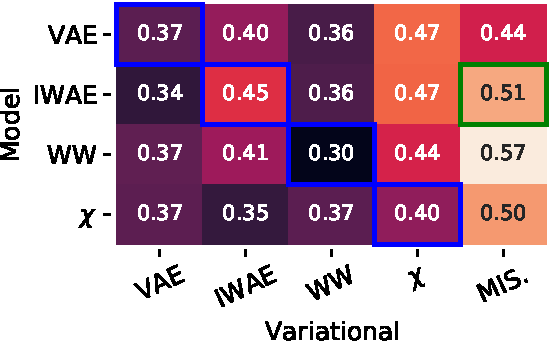
\includegraphics[width=0.4\textwidth]{figures/mnist_AUC_cross.pdf}
    \caption[AUPRC on MNIST for combinations of VAEs and inference frameworks]{AUPRC on MNIST for combinations of VAEs (row) and inference only (columns) frameworks. }\label{fig:MNIST-cross}    
\end{figure}


Table~\ref{table:m1m2} gives our results, including the Area Under the Precision-Recall Curve (AUPRC) for classifying ``nines,'' as well as goodness-of-fit metrics. IWAE and WW learn the best generative model in terms of IWELBO. For all methods, we compare the classification performance of the plugin and the SNIS estimator on labels 1 through 8. While the plugin estimator shows high accuracy across all methods (between $95\%$ and $97\%$), the SNIS estimator shows poor performance (around $60\%$). This may be because the PSIS diagnosis estimates are greater than one for all algorithms, which indicates that the variational distribution may lead to large estimation error if used as a proposal~\cite{pmlr-v80-yao18a}. 
%In this specific semi-supervised setting, the recognition model may be more representative of the conditional distribution $p(c \mid x)$ than the posterior.
%\jeff{The posterior is also a conditional distribution: the latent variables conditional on $x$. Is the posterior different than $p(c \mid x)$? Did you have $p(c, u \mid x)$ in mind as the posterior? If so, good to add that to the previous sentence.}
Consequently, we report the result of the plugin estimator for all algorithms in this experiment. Figure~\ref{fig:MNIST-cross} shows the results of applying different variational distribution for a fixed model. We also report the accuracy in Figure~\ref{fig:MNIST-acc}. These results suggest that using the $\rchi$-VAE or MIS on a fixed model leads to better decisions. In particular, our three-step procedure (IWAE-MIS) outperforms all single-proposal alternatives.

\begin{figure}
    \centering
    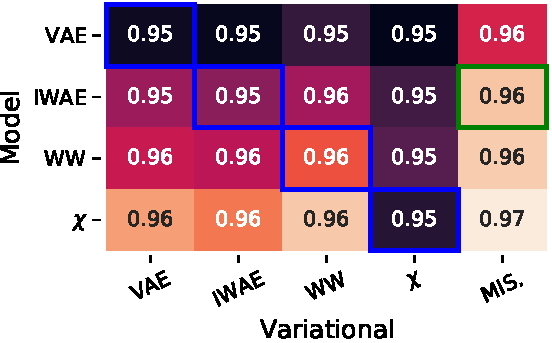
\includegraphics[width=0.4\textwidth]{figures/mnist_other_cross.pdf}
    \caption[Accuracy for M1+M2]{
    Accuracy for M1+M2: combinations of VAEs (row) and inference only (columns) frameworks. 
    }
    \label{fig:MNIST-acc}
\end{figure}
